\documentclass{beamer}
\usepackage[utf8]{inputenc}
\usepackage{graphics}
\usetheme{JuanLesPins}
\usecolortheme{crane}
\usepackage{tikz}
\usetikzlibrary{positioning}
\usepackage{xcolor}
\usepackage{adjustbox}
\usepackage{amsmath}

\title{An Introduction to Modular Arithmetic}
\subtitle{Exploration of Number Theory} 

\author{Kazi Istiak Uddin Toriqe \newline Fahad Ahmed Akash \newline Arko Sikder}
\institute[BUET]
{
    Department of CSE, BUET
}

\date{\today}
\logo{
\includegraphics[height = 1 cm]{BUET.png}} %adding logo

\begin{document}
\frame{\titlepage}

\tikzstyle{round} = [thick, blue, circle, fill = blue!20]
\tikzstyle{square} = [thick, white, rectangle, fill = green!50!blue]

\begin{frame}{}
\centering
    \begin{tikzpicture}
        \node [square] (A) {\huge \textbf {Modular}};
        \node [square] (B) [below = of A] {\huge \textbf {Arithmetic}};
    \end{tikzpicture}
\end{frame}

\begin{frame}{Think!}
    Think about a fact. When we are telling a time, we wouldn't say 13 o'clock rather we would say 1 o'clock.
    % Likewise, when we are telling 19 o'clock we would say 7 o'clock
    \newline
    \newline
    \begin{center}
        \begin{figure}
            \centering
            
\includegraphics[scale = 0.3]{think.png}
        \end{figure}
    \end{center}
\end{frame}

 \begin{frame}{Clock - 12 modulo system}
    % In our world of clocks, 16 and 4 are somehow connected. 
    % \pause 
    % In mathematics, we say - 
    \begin{columns}
        \column{0.5\textwidth}
        \newline 
        \begin{center}
        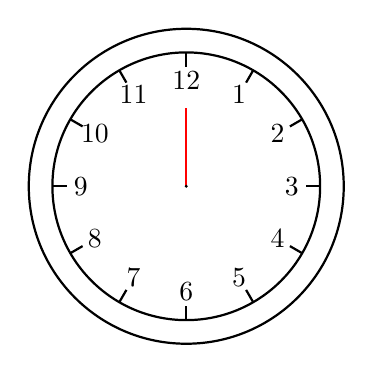
\begin{tikzpicture}[scale=2]
            % Draw the clock face
            \draw <1-> [thick] (0,0) circle (0.85);
            \draw <1-> [thick] (0,0) circle (1);
            % Draw the hour markers
            \foreach \i in {1,...,12}
                \draw  <1-> [thick] ({-(\i - 3)*(30)}:0.85) -- ({-(\i - 3)*(30)
    }:0.76) node[pos=2] {\i};
            % Draw hour hand
            \draw <1-> [thick,red] (0,0) -- ({3*30}:0.5);
            % Draw the center dot
            \fill  <1->  (0,0) circle (0.01);
        \end{tikzpicture}
        \end{center}
        \begin{alertblock}{}{\begin{center}12 o'clock\end{center}}\end{alertblock}
        \pause
        \column{0.5\textwidth}
        \begin{center}
        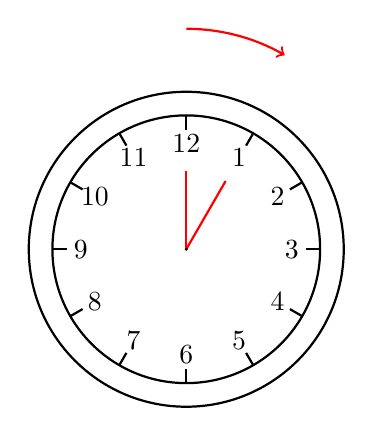
\begin{tikzpicture}[scale=2]
            % Draw the clock face
            \draw <2-> [thick] (0,0) circle (0.85);
            \draw <2-> [thick] (0,0) circle (1);
            \draw <2-> [->,red,thick] (0,1.4) arc (90:60:1.25cm);
            % Draw the hour markers
            \foreach \i in {1,...,12}
                \draw  <1-> [thick] ({-(\i - 3)*(30)}:0.85) -- ({-(\i - 3)*(30)
    }:0.76) node[pos=2] {\i};
            % Draw hour hand
            \draw <1-1> [thick,red] (0,0) -- ({3*30}:0.5);
            \draw <2-2> [thick,red] (0,0) -- ({2*30}:0.5);
            % Draw the center dot
            \fill  <2->  (0,0) circle (0.01);
        \end{tikzpicture}
        \begin{alertblock}{}{\begin{center}13 == 1 o'clock\end{center}}\end{alertblock}
        \end{center}
    \end{columns}
\end{frame}

\begin{frame}{Remainder}
    \begin{overlayarea}{\textwidth}{10cm}
    \only <1-2> {\begin{block}{} The \alert {remainder} when we divide 13 by 12 is \textbf 1. \end{block}}
    \only <3-4> { \begin{block}{} The \alert {remainder} when we divide 14 by 12 is \textbf 2. \end{block}}
    \only <5-6> {\begin{block}{}The \alert {remainder} when we divide 25 by 12 is \textbf 1.\end{block}}
        \begin{columns}
            \column{0.5\textwidth}
            \newline 
            \begin{exampleblock}
               \only <1-6> {$$ 13 \equiv 1 \pmod{12} $$}
                \only <3-6> {$$ 14 \equiv 2 \pmod{12} $$}
                \only <5-6> {$$ 25 \equiv 1 \pmod{12} $$}
            \end{exampleblock}
            \column{0.5\textwidth}
            \newline 
            \begin{exampleblock}
                \only <2-6> {$$ 13 = 12 * 1 + 1 $$}
                \only <4-6> {$$ 14 = 12 * 1 + 2 $$}
                \only <6-6> {$$ 25 = 12 * 2 + 1 $$}
            \end{exampleblock}
        \end{columns}
        % \begin{align*}
        %     \textcolor{white}{13} & \textcolor{white}{\equiv 1 \pmod{12}}  &  \textcolor{white}{13}  & \textcolor{white}{= 12 * 1 + 1} \\
        %     \only<1-> {13 &\equiv 1 \pmod{12}}  &  \only<2-> {13 &= 12 * 1 + 1} \\
        %     \only<3-> {14 &\equiv 2 \pmod{12}} &  \only<4-> {13 &= 12 * 1 + 1} \\
        %     \only<5-> {25 &\equiv 1 \pmod{12}} &  \only<6->  {25 &= 12 * 2 + 1}
        % \end{align*}   
    \end{overlayarea}
\end{frame}

\tikzstyle{abc1} = [thick, red, circle, fill = red!20]
\tikzstyle{abc2} = [thick, blue, circle, fill = blue!20]

\begin{frame}{Modular Arithmetic} 
If divide \textbf {\large a} by \textbf {\large n} gets quotient \textbf {\large q} and \textcolor{red}{remainder} \textbf {\large r}
    \begin{overlayarea}{\textwidth}{6cm}
        \begin{align*}
           \textcolor{white}{13}  & \textcolor{white}{= 12 * 1 + 1} & \textcolor{white}{13} & \textcolor{white}{\equiv 1 \pmod{12}}  \\
            \only<1->{\textbf a& \textbf{= qn + r}} & \only<>{a& \equiv r(mod n)}
        \end{align*} 
    \end{overlayarea}
\end{frame}

\tikzstyle{abc3} = [thick, black, rectangle, fill = green!20]

\begin{frame}{Modular Arithmetic} 
    \begin{overlayarea}{\textwidth}{6cm}
        \begin{align*}
           \textcolor{white}{13}  & \textcolor{white}{= 12 * 1 + 1} & \textcolor{white}{13} & \textcolor{white}{\equiv 1 \pmod{12}}    \\
            \only<1->{\textbf a& \textbf{= {\textcolor{red}{q}n + \textcolor{blue}{r}}}} & \only<2->{\textbf{a}& \equiv \textbf{r} {\textbf{(mod n)}}}
        \end{align*} 
        \only <1->{\begin{tikzpicture}
            \node [abc1] (A) {quotient};
             \node [abc2] (B) [right = of A] {remainder};
             \draw[->] (A) -- ++(42:2.5);
             \draw[->] (B) -- ++(87:1.6);
             \pause
             \node [abc3](C) [right = of B] {a is congruent to r mod n};
        \end{tikzpicture}}
    \end{overlayarea}
\end{frame}

\begin{frame}{Residue}
    Remainder r often referred to as \textcolor{red}{Residue}. A small amount of something that remains after the main part has been taken is called residue.
\end{frame}

\begin{frame}{Residue}
    \begin{figure}
        \centering
        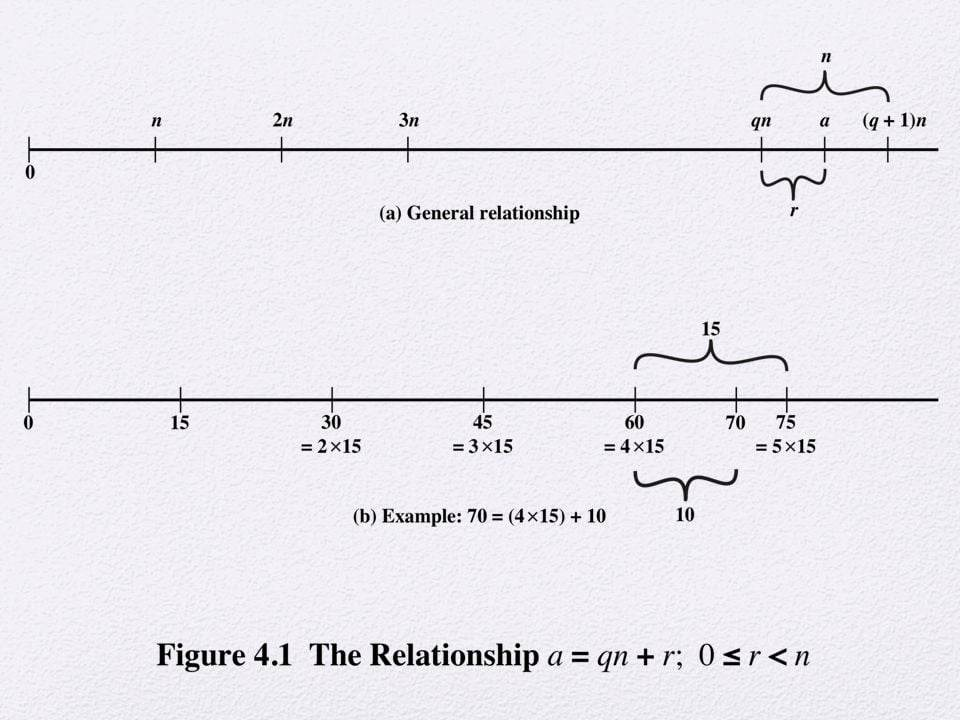
\includegraphics[scale = 0.28]{residue.jpg}
    \end{figure}
\end{frame}

% ------------
\begin{frame}{Think!}
    Now it is time to explore some properties!
    % Likewise, when we are telling 19 o'clock we would say 7 o'clock
    \newline
    \newline
    \begin{center}
        \begin{figure}
            \centering
            \includegraphics[scale = 0.3]{think2.jpg}
        \end{figure}
    \end{center}
\end{frame}

\tikzstyle{round} = [thick, blue, circle, fill = blue!20]
\tikzstyle{square} = [thick, white, rectangle, fill = green!50!blue]
\tikzstyle{x} = [circle, radius = 4 cm ]

\begin{frame}{Properties}
  \begin{center}
    \begin{tikzpicture}[>={Stealth},scale = 0.9]
        \node[thick,draw, circle, orange, radius = 4] (1) at (0, 0) {};
        \node[thick,draw, circle, orange,radius = 4] (2) at (1, 0) {};
        \node[thick,draw, circle, orange,radius = 4] (3) at (-0.5, 1) {};
        \node[thick,draw, circle, orange,radius = 4] (4) at (0.5, 1) {};
        \node[thick,draw, circle, orange,radius = 4] (5) at (1.5, 1) {};
        
        \node[thick,draw, circle, orange, radius = 4] (a) at (4, 1) {};
        \node[thick,draw, circle, orange,radius = 4] (b) at (3, 1) {};
        \node[thick,draw, circle, orange,radius = 4] (c) at (3.5, 0) {};
        
        \draw[thick,green](2.5,1.5) rectangle (4.5,-0.5);
        
        \node[thick,draw, circle, purple ,radius = 4] (t) at (6, 0.5) {};
        \node[thick,draw, circle, purple ,radius = 4] (p) at (7, 0.5) {}; 
    \end{tikzpicture}
    
    \only <2->
       {\begin{block}{}
            {$$ 5 \equiv 2 \pmod{3} $$}
        \end{block}}
    \only <3-> 
    {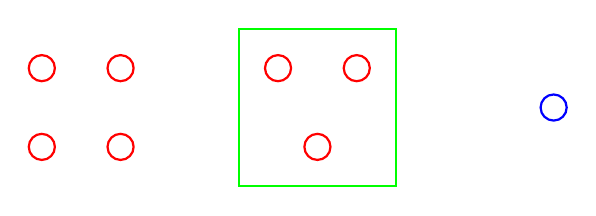
\begin{tikzpicture}
        \node[thick,draw, circle, red ,radius = 4] (6) at (0, -2) {};
        \node[thick,draw, circle, red,radius = 4] (7) at (1, -2) {};
        \node[thick,draw, circle, red ,radius = 4] (8) at (0, -3) {};
        \node[thick,draw, circle, radius = 4,red] (9) at (1, -3) {};
        
        \node[thick,draw, circle, red ,radius = 4] (6) at (4, -2) {};
        \node[thick,draw, circle, red ,radius = 4] (8) at (3, -2) {};
        \node[thick,draw, circle, radius = 4,red] (9) at (3.5, -3) {};
        \draw[thick,green](2.5,-1.5) rectangle (4.5,-3.5);
        \node[thick,draw, circle, blue ,radius = 4] (q) at (6.5, -2.5) {};
    \end{tikzpicture}}
    \only <4->
    {\begin{block}{}
            {$$ 4 \equiv 1 \pmod{3} $$}
        \end{block}}
  \end{center}
\end{frame}

\begin{frame}{Add}
  \begin{center}
    \begin{tikzpicture}[>={Stealth},scale = 0.9]
        \node[thick,draw, circle, orange, radius = 4] (1) at (-2, 0) {};
        \node[thick,draw, circle, orange,radius = 4] (2) at (-1, 0) {};
        \node[thick,draw, circle, orange,radius = 4] (3) at (-2.5, 1) {};
        \node[thick,draw, circle, orange,radius = 4] (4) at (-1.5, 1) {};
        \node[thick,draw, circle, orange,radius = 4] (5) at (-0.5, 1) {};
        
        \node[thick,draw, circle, red ,radius = 4] (6) at (0.5, 0) {};
        \node[thick,draw, circle, red,radius = 4] (7) at (1.5, 0) {};
        \node[thick,draw, circle, red ,radius = 4] (8) at (0.5, 1) {};
        \node[thick,draw, circle, radius = 4,red] (9) at (1.5, 1) {};
        
        \node[thick,draw, circle, orange, radius = 4] (a) at (3.5, 1) {};
        \node[thick,draw, circle, orange,radius = 4] (b) at (2.5, 1) {};
        \node[thick,draw, circle, orange,radius = 4] (c) at (3, 0) {};
        
        \node[thick,draw, circle, red ,radius = 4] (6) at (6, 1) {};
        \node[thick,draw, circle, red ,radius = 4] (8) at (5, 1) {};
        \node[thick,draw, circle, radius = 4,red] (9) at (5.5, 0) {};
        \draw[thick,green](2,1.5) rectangle (4,-0.5);
        \draw[thick,green](4.5,1.5) rectangle (6.5,-0.5);
        
        \node[thick,draw, circle, purple ,radius = 4] (t) at (7.5, 1) {};
        \node[thick,draw, circle, purple ,radius = 4] (p) at (8.5, 1) {}; 
        \node[thick,draw, circle, blue ,radius = 4] (q) at (8, 0) {};
        \draw[thick,blue](7,1.5) rectangle (9,-0.5);
    \end{tikzpicture}
    \only <2-2> {
        \begin{alertblock}{}
            $$Add$$
        \end{alertblock}}  
    \only <2-2> {
        \begin{block}{}
            $$ 9 \equiv 0 \pmod{3} $$
        \end{block}}
  \end{center}
\end{frame}

\begin{frame}{Sub}
    \begin{center}
        \only <1->
        \begin{tikzpicture}[>={Stealth},scale = 0.9]
            \node[thick,draw, circle, orange, radius = 4] (1) at (-2, 0) {};
            \node[thick,draw, circle, orange,radius = 4] (2) at (-1, 0) {};
            \node[thick,draw, circle, orange,radius = 4] (3) at (-2.5, 1) {};
            \node[thick,draw, circle, orange,radius = 4] (4) at (-1.5, 1) {};
            \node[thick,draw, circle, orange,radius = 4] (5) at (-0.5, 1) {};
            
            \node[thick,draw, circle, red ,radius = 4] (6) at (0.5, 0) {};
            \node[thick,draw, circle, red,radius = 4] (7) at (1.5, 0) {};
            \node[thick,draw, circle, red ,radius = 4] (8) at (0.5, 1) {};
            \node[thick,draw, circle, radius = 4,red] (9) at (1.5, 1) {};
             
            \node[thick,draw, circle, red ,radius = 4] (q) at (8, 0) {};
            % \draw[thick,blue](7,1.5) rectangle (9,-0.5);
        \end{tikzpicture}
        \only <2-2> {
            \begin{alertblock}{}
                $$Sub$$
            \end{alertblock}}  
        \only <2-2> {
            \begin{block}{}
                $$ 1 \equiv 1 \pmod{3} $$
            \end{block}}
    \end{center}
\end{frame}

\begin{frame}{Addition and Subtraction}
    \newline
    \begin{exampleblock}{}
        {$$ a_1 \equiv b_1 \pmod{m} $$}
        {$$ a_2 \equiv b_2 \pmod{m} $$}
    \end{exampleblock}
    
    \begin{columns}
        \column{0.5\textwidth}
        \begin{block}{}
            {$$ a_1+a_2 \equiv (b_1+b_2) \pmod{m} $$}
        \end{block}
    
        \column{0.5\textwidth}
        \begin{block}{}
            {$$ a_1-a_2 \equiv (b_1-b_2) \pmod{m} $$}
        \end{block}  
    \end{columns}
\end{frame}

\begin{frame}{Proof}
    \newline
    \begin{columns}
        \column{0.5\textwidth}
            \only <1-> {$$ a_1 \equiv b_1 \pmod{p} $$}
            \only <2> {$$\boldsymbol{a_1 = mp + b_1}$$}
            \only <3-> {$$a_1 = mp + b_1$$}
        \column{0.5\textwidth}
            \only <3-> {$$ a_2 \equiv b_2 \pmod{p} $$}
            \only <4> {$$\boldsymbol{a_2 = np + b_2}$$}
            \only <5-> {$$a_2 = np + b_2$$}
    \end{columns}
    \vspace{4mm}
    \begin{align*}
        \only <5-> {a_1 \pm a_2 &= (mp+b_1) \pm (np+b_2)} \\
        \only <6->          {&= (m\pm n)p + (b_1\pm b_2)} \\
        \only <7-> {X &= Ap + Y}
    \end{align*}
    \vspace{2mm}
    \only <8-> {$$ X \equiv Y \pmod{p} $$}
    \vspace{1mm}
    \only <9-> {$$ a_1\pm a_2 \equiv (b_1\pm b_2) \pmod{p} \hspace{0.5cm} \textbf{[QED]} $$}
\end{frame}


\section{Multiplication}
\begin{frame}{Multiplication}
    \vspace{0.5cm}
    \begin{block}{}
        \only <1-> {$$ 5 \equiv 2 \pmod{3} $$}
        \only <1-> {$$ 4 \equiv 1 \pmod{3} $$}
    \end{block}
    \vspace{1cm}
    \only <2-> {\begin{alertblock}{}
        {$$Multiply$$}  
    \end{alertblock}}
    \only <2-> {\begin{block}{}
         {$$ 20 \equiv 2 \pmod{3} $$}
    \end{block}}
\end{frame}

\begin{frame}{Multiplication}
    \vspace{0.2cm}
    \begin{block}{}
        {$$ a_1 \equiv b_1 \pmod{m} $$}
        {$$ a_2 \equiv b_2 \pmod{m} $$}
    \end{block}
    \vspace{1cm}
    \par
    \begin{alertblock}{}
         \centerline{\boldsymbol{$$ a_1a_2 \equiv b_1b_2 \pmod{m} $$}}
    \end{alertblock}
    \only <2-> {\centerline{Can be easily proved just as before!}}
\end{frame}


\begin{frame}{Power}
    \vspace{0.2cm}
    {$$ a_1a_2 \equiv b_1b_2 \pmod{m} $$}
    \vspace{0.3cm}
    \only <2->
    {\par
    If we put $a_1=a_2=a$,
    \newline
    {$$ a^2 \equiv b^2 \pmod{m} $$}}
    \vspace{0.1cm}
    \only <3->
    {\par
    If we keep multiplying,}
    \only <4->
    {\newline
    \begin{alertblock}{}
        {$$ a^n \equiv b^n \pmod{m} $$}
    \end{alertblock}
    }
    
\end{frame}

\begin{frame}{An Interesting Problem}
    \vspace{0.2cm}
    \begin{block}{}
        {Find the last digit of $(2+0+2+3)^{2023}$}
    \end{block}
    \newline
    \newline
    \only <2->
    {$Sol^n:$
    \begin{align*}
        {7^{2023}}
        \only <3-> {&\equiv 7^{2022}\cdot 7 \pmod{10}} \\
        \only <4-> {&\equiv (7^{2})^{1011}\cdot 7 \pmod{10}} \\
        \only <5-> {&\equiv (49)^{1011}\cdot 7 \pmod{10}} \\
        \only <6-> {&\equiv (-1)^{1011}\cdot 7 \pmod{10}} \\
        \only <7-> {&\equiv (-1)\cdot 7 \pmod{10}} \\
        \only <8-> {&\equiv -7 \pmod{10}} \\
        \only <9-> {&\equiv 3} \\
    \end{align*}}
    \only <10->
    {\par
    {So the last digit of $7^{2023}$ is 3}}
\end{frame}


% ----------


\begin{frame}{\textbf{Modular Arithmetic for Division}}
    \only<1-1> {
    \begin{center}
        \begin{figure}
            \centering
            
\includegraphics[scale = 0.3]{think.png}
        \end{figure}
    \end{center}}
    
    \only<3-3> {
    \begin{center}
        \begin{figure}
            \centering
            
\includegraphics [scale = 0.1]{anger1.jpg}
        \end{figure}
    \end{center}}
    \begin{center}
        \begin{itemize}
            \item <1-> Can we do modular operations for division algorithms ? 
            \item <2-> The answer is no . Division algorithm doesn't work like that way all the time .
            \item <3-> Why ?
            \item <4->Remember what we know !! we cannot divide anything by $0$ .
            \item <5->Even if , $a\equiv 0 \pmod b$
        \end{itemize}
    \end{center}
\end{frame}

\begin{frame}{\textbf{Modular Arithmetic for Division}}
    \begin{center}
        \begin{itemize}
            \item <1-> We can't determine it simply by writing
    \end{itemize} 
       \begin{block}{}
           $$ (\frac{a}{b}) \equiv \frac{a \equiv d_1 \pmod m}{b \equiv d_2 \pmod m} $$
       \end{block} 
        \begin{itemize}
            \item <2-> 
                Because there's a possibility of the denominator $ d_2 $ becoming 0 again!!
        \end{itemize} 
    \end{center}  
    \newline
    \newline
\end{frame}

\begin{frame}{\textbf{Modular Arithmetic for Division}}
    \begin{itemize}
        \item <1->Let's see another example for more clear picture 
        \newline 
        \begin{equation}
            15 \equiv 6 \pmod 9 
        \end{equation}
        \begin{equation}
            3 \equiv 3 \pmod 9
        \end{equation}
        
        \item <2->if we use the distribution law for division , We will get $$ 5 \equiv 2 \pmod 9 $$
        \newline
        \item <3->Which emerges a disastrous question to our knowledge about division !!
    \end{itemize}
    \newline
    \only<3->{
    \begin{center}
        \textbf{How do we know it ?}
    \end{center}
    }
\end{frame}
\begin{frame}{\textbf{Modular Multiplicative Inverse}} 
    \only <1-> {$$5 . 5^{-1} \equiv 1 \pmod 9$$}
    \newline
    \only <2-> {$$\Rightarrow 5b \equiv 1\pmod 9 $$}
    \newline
    \only <3-> {$$\Rightarrow 5.2 \equiv 1\pmod 9 $$}
    \newline
    \only <4-> {$\textbf{2}$ is the modular multiplicative inverse of $\textbf{5},$ modulo $\textbf{9}$}
    \begin{center}
    \end{center}
\end{frame}

\begin{frame}{\textbf{Modular Multiplicative Inverse}} 
    Let's Solve a problem !
    \begin{center}
    \begin{block}{}
        $$(\frac{20}{5}) \pmod 9$$
    \end{block}
    \end{center}
    \newline
    \only<2->{$\textbf{2}$ is the modular multiplicative inverse of $\textbf{5},$ modulo $\textbf{9}$
    $$20.\frac{1}{5} \equiv (20*2)\equiv 4 \pmod 9$$}
    \newline
    \begin{center}
        \begin{itemize}
            \item<3-> $ab \equiv 1 \pmod p$ and $\textbf{gcd(a,p)} = 1$
            \item<4-> $\textbf{b}$ is called the modular multiplicative inverse of $\textbf{a}$ modulo $\textbf{p}$
        \end{itemize}
    \end{center}
\end{frame}

\begin{frame}{\textbf{Modular Multiplicative Inverse}}
    \begin{center}
        \begin{itemize}
            \item <1->A modular multiplicative inverse of a positive integer $\textbf{a}$ modulo $\textbf{p}$ is always unique
            \item <2->Otherwise $\textbf{a}$ and $\textbf{b}$ must not be   relatively-prime 
        \end{itemize}
    \end{center}
    \only <3-> {\textbf{Proof :}}
    \begin{center}
        \begin{itemize}
            \item <3->suppose $\exists \textbf{c} \in Z^{+} , \textbf{c}$ is a solution 
            \item <4->$ab \equiv ac \equiv 1 \pmod p$
            \item <5->$a(b-c)\equiv 0 \pmod p$
        \end{itemize}
    \end{center}
\end{frame}

\begin{frame}{\textbf{Modular Multiplicative Inverse}}
    \textbf{Proof Continues :}
    \begin{center}
        \begin{itemize}
            \item <1-> Either $a\equiv 0 \pmod p$
            \item <2-> or $(b-c) \equiv 0 \pmod p$
            \item <3-> $a\equiv 0 \pmod p$
            \item<4-> Therefore $gcd(a,p) \neq 1 $ which is a contradiction
            \item<5-> So, $(b-c) \equiv 0 \pmod p$
            \item<6-> $b = c \pmod p$
        \end{itemize}
    \end{center}
\end{frame}

\begin{frame}{Exercise}
    Some interesting problem may become food for your brain!
    \begin{itemize}
        \item Josephus problems
        \item Extended GCD
    \end{itemize}
    Recommended books -
    \begin{itemize}
        \item Art and Craft of Problem Solving
        \item 102 Number Theory Problems
    \end{itemize}
\end{frame}

\begin{frame}{Q/A}
\begin{block}{}
\begin{center}
   \huge { Questions? }
\end{center}
\end{block}
\end{frame}

\begin{frame}{Thank you!}
    \begin{figure}
        \centering
        
\includegraphics[scale = 0.1]{Thankyou.jpg}
    \end{figure}
\end{frame}
\end{document}